\documentclass[a4paper,12pt]{report}
\usepackage[utf8]{inputenc}
\usepackage[T1]{fontenc}
\usepackage[french]{babel} 
\usepackage{xcolor,graphicx}
\usepackage{enumitem}
\usepackage{hyperref}
\usepackage[margin=0in]{geometry}
\graphicspath{{image/}}
\usepackage{graphicx}
\usepackage{array}

\begin{document}


\underline{\textbf{LES DIFFERENTS CAPTEURS}}\\ \break
\setlength{\indent}
Il y a les capteurs \underline{\textbf{piézo-résistifs}}, \underline{\textbf{capacitifs}},et \underline{\textbf{electro-mécanique}}.  

\hfill

\begin{itemize} 
\setlength{\itemindent}{1cm}
 \item \underline{\textbf{BMP180:}}
\end{itemize}

\setlength{\itemindent}{3cm}

Le BMP180 est composé principalement d'un \underline{capteur piézo-résistif},d'un \underline{convertisseur analogique vers digital} 
et \\ une \underline{unité de contrôle composé d'un EEPROM et de l'interface I2C série}.\\

Ce capteur est designé pour être \textbf{directement connecté au microcontrôlleur} grâce au bus I2C. 

\begin{itemize}

\setlength{\itemindent}{2cm}
\item \underline{\textit{\textbf{Principe de fonctionnement:}}} Comme le capteur à une "unité de
 contrôle" elle lui permet de mesurer la pression après un laps de temps donné et d'avoir le résultat des calculs.    
\end{itemize} 


\centering
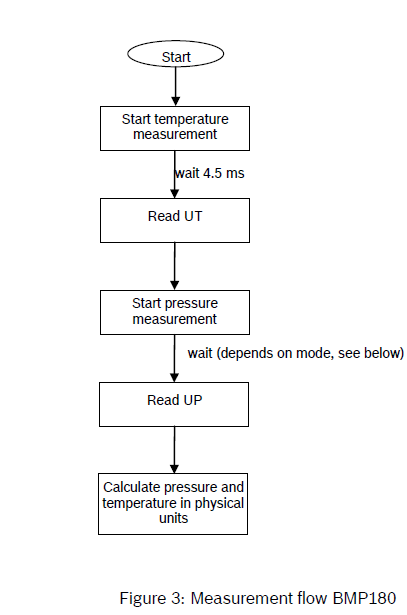
\includegraphics[width=0.35\textwidth]{2.png}
\hspace{2cm} 
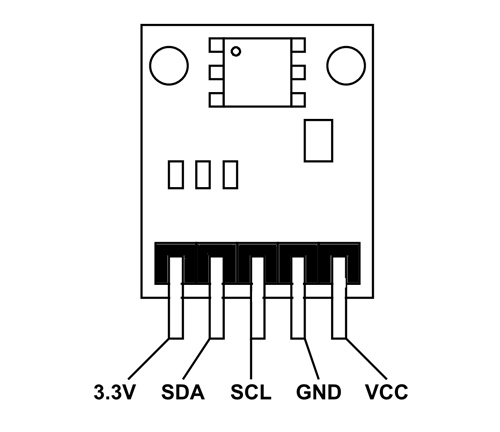
\includegraphics[width=0.20 \textwidth]{BMP180-Sensor-Pinout.png}
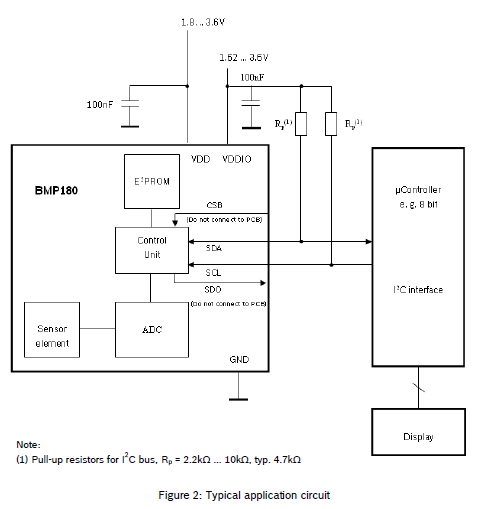
\includegraphics[width=0.50\textwidth]{sblck.png}

\vspace{3cm}
\hfill

\begin{itemize}
\vspace{2cm}
\setlength{\itemindent}{2cm}
\item \underline{\textit{\textbf{Plage de valeurs mesurée:}}} L'intervalle est de \textbf{300} à \textbf{1100hPa} (110.000 Pa)
\end{itemize} 

\begin{itemize}
\setlength{\itemindent}{2cm}
\item \underline{\textit{\textbf{Tension d'alimentation:}}} Entre \textbf{1.8} à \textbf{3.6V} 
\end{itemize} 

\vspace{1cm}

\begin{itemize} 
\setlength{\itemindent}{1cm}
 \item \underline{\textbf{MPX4115A:}}
\end{itemize}

\setlength{\itemindent}{3cm}

Le MPX4115A est un capteur piézo-résistifs de pression absolue.\\

\begin{itemize}

\setlength{\itemindent}{2cm}
\item \underline{\textit{\textbf{Principe de fonctionnement:}}} 
Le capteur calcul la pression à l'aide de cette formule présente dans le datasheet :\\   \fbox{$V_{out} = V_s * (0.009P - 0.95)$}  \\
 où : \\ $V_{out}$ désigne la tension de sortie \\ $V_s$ la tension d'entrée \\ $P$ la pression mesurée 


\end{itemize} 

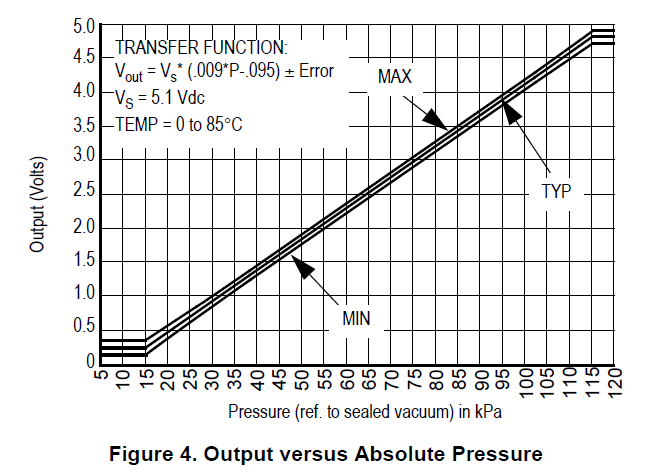
\includegraphics[width=0.70\textwidth]{3.png}
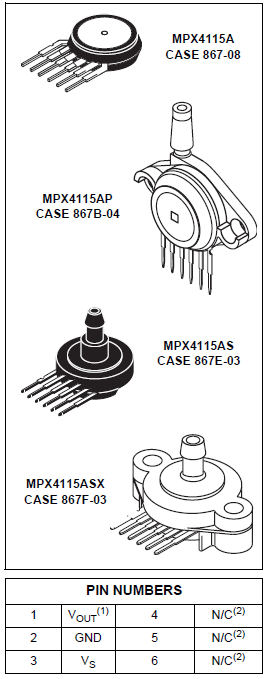
\includegraphics[width=0.25\textwidth]{4.png}


\begin{itemize}
\vspace{2cm}
\setlength{\itemindent}{2cm}
\item \underline{\textit{\textbf{Plage de valeurs mesurée:}}} L'intervalle est de \textbf{15} à \textbf{115kPa} (115.000 Pa)
\end{itemize} 


\begin{itemize}
\setlength{\itemindent}{2cm}
\item \underline{\textit{\textbf{Tension d'alimentation:}}} Entre \textbf{4.85} à \textbf{5.35V} 
\end{itemize}

\vspace{5cm}

\begin{itemize}
\break
\setlength{\itemindent}{1cm}
 \item \underline{\textbf{BMP280:}}
\end{itemize}

\begin{itemize}

\setlength{\itemindent}{2cm}
\item \underline{\textit{\textbf{Principe de fonctionnement:}}} Il utilise le même principe que son prédecesseur le \underline{\textbf{BMP180}}
 mais est \underline{\textbf{ plus précis}}, et peut mesurer la température et l'altitude.
\end{itemize} 

\begin{itemize}
\setlength{\itemindent}{2cm}
\item \underline{\textit{\textbf{Plage de valeurs mesurée:}}} L'intervalle est de \textbf{300hPa} à \textbf{1110hPa} (111.000 Pa)
\end{itemize} 


\begin{itemize}
\setlength{\itemindent}{2cm}
\item \underline{\textit{\textbf{Tension d'alimentation:}}} Entre \textbf{1.8} à \textbf{3.6V} 
\end{itemize} 

\vspace{1.5cm}

\underline{\textbf{COMPARATIFS DES CAPTEURS}}

\begin{table}[h!]
\centering
\begin{tabular}{|>{\raggedright\arraybackslash}m{3cm}|>{\raggedright\arraybackslash}m{3cm}|>{\raggedright\arraybackslash}m{3cm}|>{\raggedright\arraybackslash}m{3cm}|}
\hline
\textbf{Critère} & \textbf{BMP180} & \textbf{BMP280} & \textbf{MPX4115A} \\
\hline
\textbf{Plage de Pression} & 300 à 1100 hPa & 300 à 1100 hPa & 15 à 115 kPa  \\
\hline
\textbf{Précision} & ±1 hPa & ±1 hPa & ±1.5 \% de la pleine échelle \\
\hline
\textbf{Tension d'Alimentation} & 1.8V à 3.6V & 1.8V à 3.6V & 4.85V à 5.35V \\
\hline
\textbf{Consommation Énergétique} & 3.4 µA & 2.7 µA & Typiquement 7 mA \\
\hline
\textbf{Interface de Communication} & I2C, SPI & I2C, SPI & Sortie analogique \\
\hline
\textbf{Température de Fonctionnement} & -40°C à 85°C & -40°C à 85°C & -40°C à 125°C \\
\hline
\textbf{Dimensions Physiques} & 3.6 x 3.8 x 0.93 mm & 2.0 x 2.5 x 0.95 mm & 7.6 x 7.9 x 4.8 mm \\
\hline
\textbf{Coût} & Abordable & Légèrement plus cher & Le plus cher des 3 \\
\hline
\end{tabular}
\end{table}



\end{document}
